The \emph{visible cross section} is defined as:
\begin{equation}
  \label{eq:90}
  \sigma_\mathrm{\, vis} = \sigma \times A \times \epsilon
\end{equation}
where $\sigma$ is the production cross section, $A$ is the selection acceptance
and $\epsilon$ is the selection efficiency. The CL$_\mathrm{\, S}$ modified
frequentist approach mentioned in Section~\ref{sec:sign-hypoth-excl} is used to
set 95\% CL exclusion limit on the \emph{visible cross section} for models with
a monojet final state experimental signature. The results are reported in
Table~\ref{tab:cs_vis_results}, values of $\sigma_\mathrm{\, vis}$ above
$\langle \sigma \rangle_\mathrm{\, obs}^{\, 95}$ ($\sigma_\mathrm{\, vis}$ >
$\langle \sigma \rangle_\mathrm{\, obs}^{\, 95}$) are excluded at 95\%
CL. Figure~\ref{fig:sr_plots}, reports the distribution of the measured $\met$
and the leading jet $\pt$ in the SR\@. There is a good agreement between data
and SM predictions, the latter is normalized using the results of the global fit
in the exclusive $\met$ regions (EM1--EM6).

\begin{figure}[!th]
  \centering
  \begin{subfigure}[t]{.48\linewidth}
    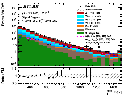
\includegraphics[width=\linewidth]{sr_et_miss}
    \caption{$\met$ distribution.}
    \label{fig:sr_et_miss}
  \end{subfigure}
  \begin{subfigure}[t]{.48\linewidth}
    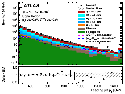
\includegraphics[width=\linewidth]{sr_jet1_pt}
    \caption{Leading jet $\pt$ distribution.}
    \label{fig:sr_jet1_pt}
  \end{subfigure}
  \caption{Distribution of the $\met$ and the leading jet $\pt$ for IM1 signal
    region compared with the normalized SM predictions. The distributions of
    different signal models are superimposed for comparison. The contribution
    from the multi-jet and NCB background is negligible and not reported in the
    plot. In the ratio window the error bars include experimental and systematic
    uncertainties.}
  \label{fig:sr_plots}
\end{figure}

\begin{table}[!h]
  \centering
  \begin{tabular}{llll}
    \toprule
    \multicolumn{4}{c}{Result Table} \\
    \midrule \midrule
    Signal Region & $\langle \sigma \rangle_\mathrm{\, obs}^{\, 95}$ [fb] & S$_\mathrm{\, obs}^{\, 95}$ & S$_\mathrm{\, exp}^{\, 95}$ \\
    \midrule
    IM1 & 533 & 1773 & 1864$_{\, -548}^{\, +829}$ \\
    IM2 & 308 & 988 & 1178$_{\, -348}^{\, +541}$ \\
    IM3 & 196 & 630 & 694$_{\, -204}^{\, +308}$ \\
    IM4 & 153 & 491 & 401$_{\, -113}^{\, +168}$ \\
    IM5 & 61 & 196 & 164$_{\, -45}^{\, +63}$ \\
    IM6 & 23 & 75 & 84$_{\, -23}^{\, +32}$ \\
    IM7 & 19 & 61 & 48$_{\, -13}^{\, +18}$ \\
    \bottomrule
  \end{tabular}
  \caption{Results on the expected and observed upper limits on the number of events and on the
    visible cross section at 95\% CL.}
  \label{tab:cs_vis_results}
\end{table}
%%% Local Variables:
%%% mode: latex
%%% TeX-master: "../search_for_DM_LED_with_ATLAS"
%%% End:
